%%This is a very basic article template.
%%There is just one section and two subsections.
\documentclass{article}

\usepackage{graphicx}
\usepackage{listings}
\usepackage{color}
\usepackage{makeidx}
\usepackage{hyperref}
\usepackage{parskip}
\usepackage{multirow}

\makeindex

\hypersetup{
    %bookmarks=true,         % show bookmarks bar?
    unicode=false,          % non-Latin characters in Acrobat’s bookmarks
    pdftoolbar=true,        % show Acrobat’s toolbar?
    pdfmenubar=true,        % show Acrobat’s menu?
    pdffitwindow=false,     % window fit to page when opened
    pdfstartview={FitH},    % fits the width of the page to the window
    pdftitle={TDT4205 Compilers - Exercise 3 - hvatum},    % title
    pdfauthor={Stian Hvatum},     % author
    pdfsubject={TDT4205 Compilers},   % subject of the document
    pdfcreator={Stian Hvatum},   % creator of the document
    pdfproducer={Stian Hvatum}, % producer of the document
    pdfnewwindow=true,      % links in new window
    colorlinks,       % false: boxed links; true: colored links
    linkcolor=red,          % color of internal links
    citecolor=green,        % color of links to bibliography
    filecolor=magenta,      % color of file links
    urlcolor=cyan           % color of external links
}

\lstset{ %
  literate= {+}{{$+$}}1 {*}{{$*$}}1 {=}{{$\gets$}}1 
            {<=}{{$\leq$}}1 {>=}{{$\geq$}}1 {!=}{{$\neq$}}1 
            {==}{{$\equiv$}}1 {=>}{{$\leadsto$}}1
            {->}{{$\rightarrow$}}1
}

\definecolor{listinggray}{gray}{0.9}
\definecolor{lbcolor}{rgb}{0.9,0.9,0.9}
\lstset{
    keywordstyle=\bfseries\ttfamily\color[rgb]{0,0,1},
    identifierstyle=\ttfamily,
    commentstyle=\color[rgb]{0.133,0.545,0.133},
    stringstyle=\ttfamily\color[rgb]{0.627,0.126,0.941},
    showstringspaces=false,
    basicstyle=\tiny,
    numberstyle=\tiny,
    framexleftmargin=3pt,
    numbers=left,
    stepnumber=1,
    numbersep=15pt,
    tabsize=2,
    breaklines=true,
    prebreak = \raisebox{0ex}[0ex][0ex]{\ensuremath{\hookleftarrow}},
    breakatwhitespace=false,
    aboveskip={1.5\baselineskip},
    columns=fixed,
    upquote=true,
    extendedchars=true,
  	frame=l,
    sensitive=true,
}

\renewcommand{\thesection}{PART \arabic{section}}
\renewcommand{\thesubsection}{Task \arabic{section}.\arabic{subsection}}
\renewcommand{\thesubsubsection}{\arabic{section}.\arabic{subsection}.\arabic{subsubsection}}

\title{TDT4205 Compilers\\
\Huge Exercise 3}
\author{Stian Hvatum (hvatum)\\MTDT}

\begin{document}
\maketitle

\section{Theory}
\subsection{Parsing}
\subsubsection{LL(k)}
Even if LL(\textit{k}) in theory can be extended with an $\rightarrow infinitly$
number of lookaheads, this will not resolve the problems with left recursion. For each
lookahead-symbol extra, the parse table grows, and at the end it will become
humongous. To create and use such a table is both space and time consuming, and
we will never have neither space nor time to parse languages and grammars with arbitary use of left
recursion, as it requires arbitary much space and time. Also, LL(\textit{k}) needs the
\textit{k} to be defined, wich sets an upper bound for the number of lookaheads
before we begin parsing. We may set the \textit{k} to 10000000000, and hope that
the language will never exeed this number of recursions, but it will not be a
\emph{valid} parser for that language, as it can only handle a subset of the
possible language constructs.

\subsubsection{Left-recursive grammars}
The left-recursive grammar:\\
\begin{tabular}{ccl}
F & $\rightarrow$ & f I v A w S x \\ 
A & $\rightarrow$ & P \\
P & $\rightarrow$ & P I $| \epsilon$\\ 
S & $\rightarrow$ & S s $|$ s\\
I & $\rightarrow$ & i\\
\end{tabular}


The equivalent non-left-recursive grammer:\\
\begin{tabular}{ccl}
F & $\rightarrow$ & f I v A w S x \\ 
A & $\rightarrow$ & P \\
P & $\rightarrow$ & I P $| \epsilon$\\ 
S & $\rightarrow$ & s S'\\
S' & $\rightarrow$ & s S' $| \epsilon$\\
I & $\rightarrow$ & i\\
\end{tabular}

\subsubsection{{\ttfamily FIRST} and {\ttfamily FOLLOW} \& LL(1) Parsing table}
\subsubsection*{{\ttfamily FIRST} and {\ttfamily FOLLOW}}
Computing {\ttfamily FIRST}
\begin{itemize}
  \item f is in FIRST(F), since f is the first symbol in production of F, and f
  is a terminal, and thereby FIRST(f) = f.
  \item i is in FIRST(I), since FIRST(I) = FIRST(i) = i
  \item i is in FIRST(P), since FIRST(P) = FIRST(I) = i 
  \item $\epsilon$ is in FIRST(P), since P has a production P $\rightarrow
  \epsilon$
  \item i, $\epsilon$ is in FIRST(A), since FIRST(A) = FIRST(P) = i, $\epsilon$
  \item s is in FIRST(S) since FIRST(S) = FIRST(s) = s 
  \item s is in FIRST(S') since FIRST(S') = FIRST(s) = s 
  \item $\epsilon$ is in FIRST(S'), since S' has a production S' $\rightarrow
  \epsilon$
\end{itemize}
Computing {\ttfamily FOLLOW}
\begin{itemize}
  \item We start by adding \$ to F, since F is our \emph{start-symbol}.
  \item We see from F $\rightarrow$ f I v A w S x that w is in FOLLOW(A), x
  is in FOLLOW(S) and v is in FOLLOW(I)
  \item FOLLOW(P) = FOLLOW(A) since A $\rightarrow$ P. 
  \item FOLLOW(S') = FOLLOW(S) since S $\rightarrow$ S'.
  \item FOLLOW(I) includes FIRST(P) except $\epsilon$ since P $\rightarrow$ I P
  $| \epsilon$, and rule 3, wich makes FOLLOW(I) = i, v
\end{itemize}
\begin{tabular}{|c|c|c|c|}
\hline
NT & FIRST & FOLLOW \\
\hline
\hline
F  & f & \$ \\
A  & i, $\epsilon$ & w \\
P  & i, $\epsilon$ & w \\
S  & s & x \\
S' & s, $\epsilon$ & x \\
I  & i & i, v, w \\
\hline
\end{tabular}
\subsubsection*{LL(1) Parsing table}
Followed page 224, Alg. 4.31\\
IF A $\rightarrow$ b AND FIRST(b) contains c THEN add A $\rightarrow$ b to
M(A,c) and\\
IF FIRST(b) contains $\epsilon$, THEN add A $\rightarrow \epsilon$ to M(A,c)
M(A,b) M(A,c)\\
\begin{tabular}{|c|c|c|c|c|c|c|c|}
\hline
Non- & \multicolumn{7}{c|}{Input Symbol}\\
\cline{2-8}
Terminal & f & i & v & w & s & x & \$ \\
\hline
\hline
F  & F $\rightarrow$ f I v A w S x & & & & & & \\
\hline
A  & & A $\rightarrow$ P & & A $\rightarrow$ $\epsilon$ & & & \\
\hline
P  & & P $\rightarrow$ I P & & P $\rightarrow$ $\epsilon$ & & & \\
\hline
S  & & & & & S $\rightarrow$ sS' & & \\
\hline
S' & & & & & S' $\rightarrow$ sS' & S' $\rightarrow$ $\epsilon$ & \\
\hline
I  & & I $\rightarrow$ i & & & & & \\
\hline
\end{tabular}

\subsubsection{Parse tree for LL(1)}
\begin{tabular}{ccc}
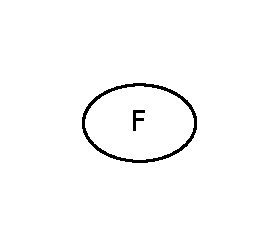
\includegraphics[width=427px]{LL1-ParseTree/1.pdf}
\includegraphics[width=427px]{LL1-ParseTree/LL1-ParseTree.pdf}
\end{tabular}

\printindex
\end{document}
